\documentclass[11pt]{article}

\usepackage[margin=1in]{geometry}
\usepackage{amsmath,amssymb,bm}
\usepackage{graphicx}
\usepackage{float}
\usepackage{placeins}
\usepackage{xcolor}
\usepackage{tikz}
\usetikzlibrary{arrows.meta,calc,fit,positioning,decorations.pathreplacing,shapes.geometric}
\usepackage{hyperref}

\definecolor{sigaBlueFill}{HTML}{E8F2FF}
\definecolor{sigaBlueLine}{HTML}{2F5F8F}
\definecolor{sigaGreenFill}{HTML}{EAF7EF}
\definecolor{sigaGreenLine}{HTML}{3F7D57}
\definecolor{sigaAmberFill}{HTML}{FFF4D6}
\definecolor{sigaAmberLine}{HTML}{9A6B16}
\definecolor{sigaTealFill}{HTML}{E6F6F4}
\definecolor{sigaTealLine}{HTML}{2A7F79}
\definecolor{sigaPurpleFill}{HTML}{F0EBFF}
\definecolor{sigaPurpleLine}{HTML}{6B5AA6}
\definecolor{sigaRoseFill}{HTML}{FDEDEE}
\definecolor{sigaRoseLine}{HTML}{A8555A}
\definecolor{sigaArrow}{HTML}{334155}

\title{Software Architecture of SIGA}
\author{}
\date{}

\begin{document}

\maketitle

\section{Software Architecture of SIGA}
\label{sec:software_architecture}

SIGA is designed as a modular GPU-accelerated isogeometric analysis framework for nonlinear and higher-gradient computational mechanics. The architecture separates the program into five major layers: geometry and spline-basis construction, degree-of-freedom and boundary-condition management, GPU-based residual and tangent assembly, sparse linear/nonlinear solution, and post-processing. This separation allows the same geometric and discretization infrastructure to be reused by several physical models, including nonlinear elasticity, strain-gradient elasticity, electroelasticity, and flexoelectricity.

Figure~\ref{fig:siga_architecture_overview} shows the main data flow in SIGA. The user first defines knot vectors, control points, material parameters, boundary conditions, and solver options. These inputs are converted into patch-level and multipatch data structures. The discretization layer constructs the spline basis, performs degree elevation or refinement, and builds the global degree-of-freedom mapping. The assembly layer then transfers the required geometry, basis, quadrature, and sparse-system information to the GPU. At each Newton iteration, SIGA evaluates the residual vector and tangent matrix on the GPU, stores the resulting sparse system in compressed sparse row format, and calls a linear solver backend. After convergence, the solution and derived quantities are reconstructed as spline fields and written to visualization files.

\begin{figure}[H]
\centering
\resizebox{\textwidth}{!}{%
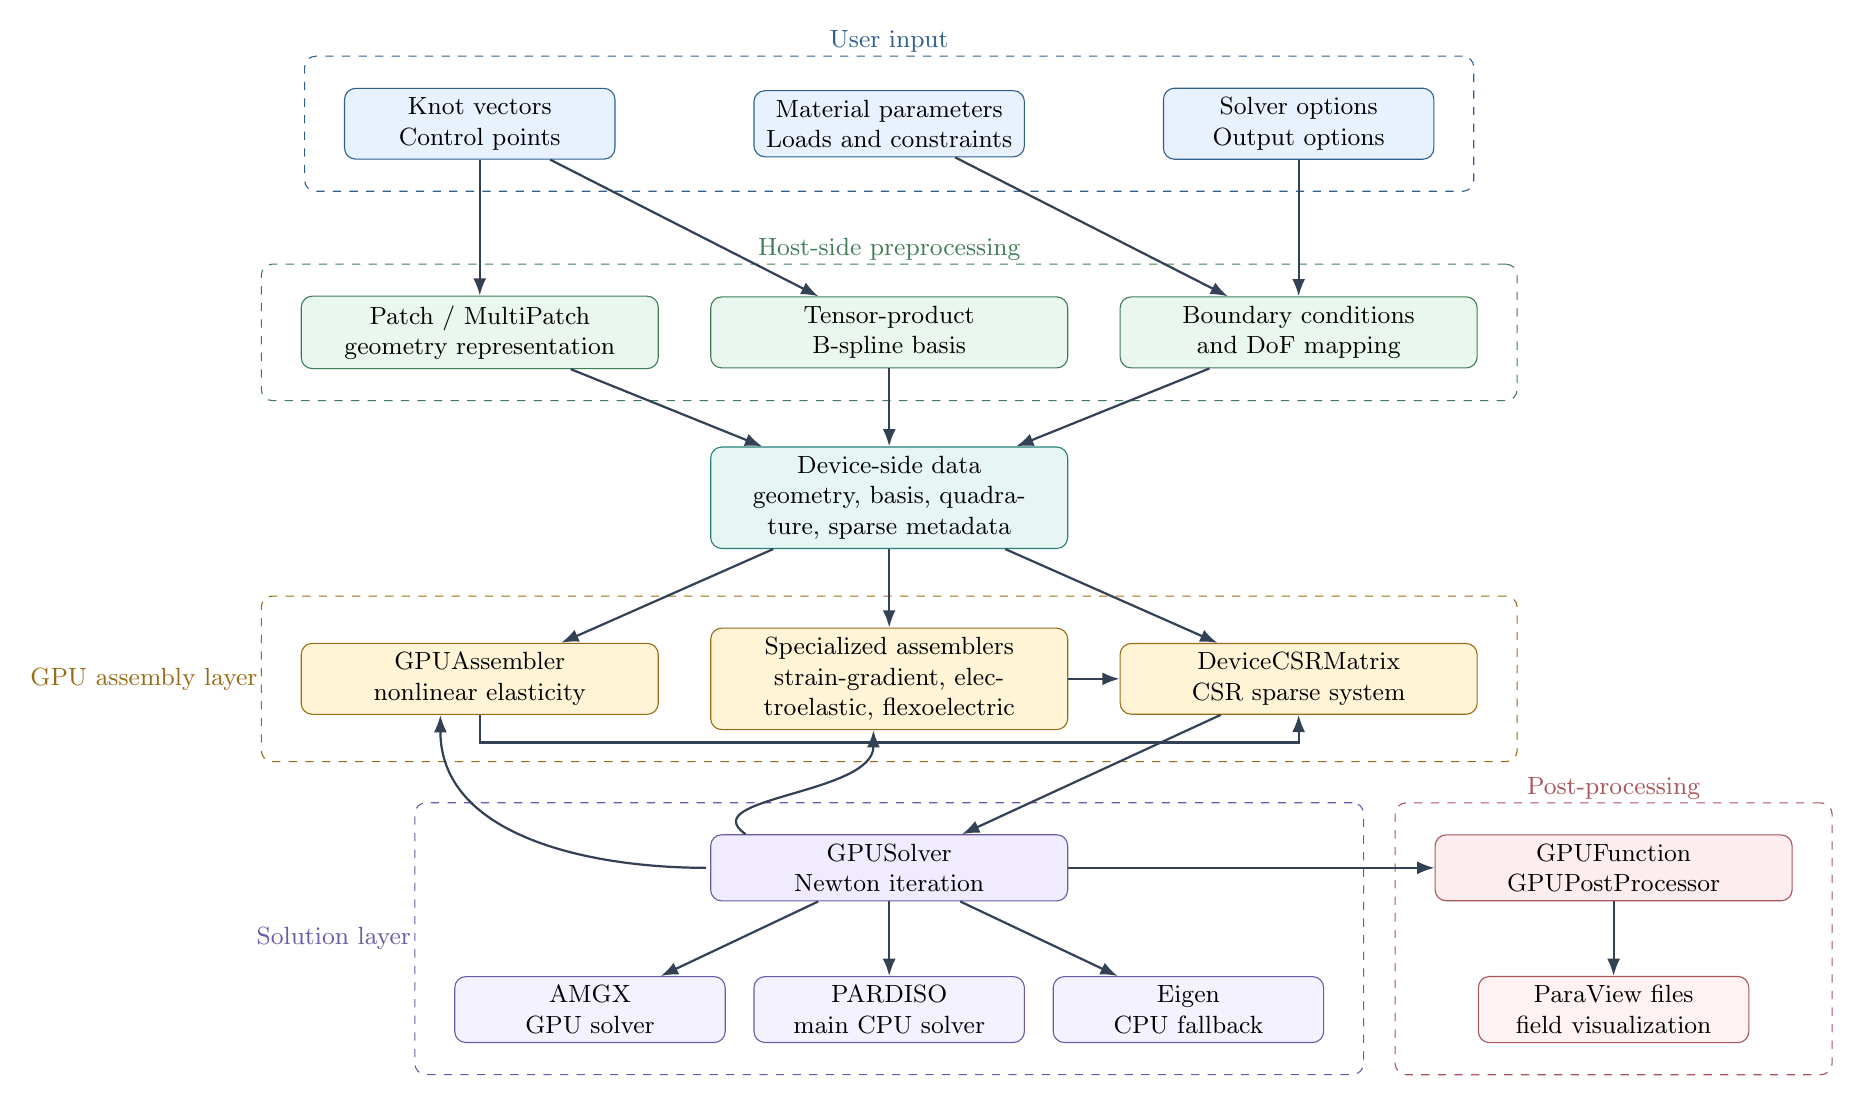
\begin{tikzpicture}[
    font=\small,
    box/.style={
        draw=sigaArrow,
        fill=white,
        rounded corners,
        align=center,
        minimum height=8mm,
        text width=32mm
    },
    widebox/.style={
        draw=sigaArrow,
        fill=white,
        rounded corners,
        align=center,
        minimum height=8mm,
        text width=43mm
    },
    inputnode/.style={box, fill=sigaBlueFill, draw=sigaBlueLine},
    preprocessnode/.style={widebox, fill=sigaGreenFill, draw=sigaGreenLine},
    devicenode/.style={widebox, fill=sigaTealFill, draw=sigaTealLine},
    assemblynode/.style={widebox, fill=sigaAmberFill, draw=sigaAmberLine},
    solvernode/.style={widebox, fill=sigaPurpleFill, draw=sigaPurpleLine},
    backendnode/.style={box, fill=sigaPurpleFill!65, draw=sigaPurpleLine},
    postnode/.style={widebox, fill=sigaRoseFill, draw=sigaRoseLine},
    postsmallnode/.style={box, fill=sigaRoseFill!75, draw=sigaRoseLine},
    groupbox/.style={
        draw=sigaArrow,
        rounded corners,
        dashed,
        inner xsep=5mm,
        inner ysep=4mm
    },
    grouplabel/.style={
        font=\small,
        fill=white,
        text=sigaArrow,
        inner sep=1pt
    },
    arrow/.style={
        -{Latex[length=2.2mm]},
        thick,
        draw=sigaArrow
    }
]

% Input layer
\node[inputnode] (input_geo) at (0,0) {Knot vectors\\Control points};
\node[inputnode] (input_phys) at (5.2,0) {Material parameters\\Loads and constraints};
\node[inputnode] (input_opts) at (10.4,0) {Solver options\\Output options};

% Geometry/discretization layer
\node[preprocessnode] (patch) at (0,-2.65) {Patch / MultiPatch\\geometry representation};
\node[preprocessnode] (basis) at (5.2,-2.65) {Tensor-product\\B-spline basis};
\node[preprocessnode] (bc) at (10.4,-2.65) {Boundary conditions\\and DoF mapping};

% Device data layer
\node[devicenode] (device) at (5.2,-4.75) {Device-side data\\geometry, basis, quadrature, sparse metadata};

% Assembly layer
\node[assemblynode] (assembler_base) at (0,-7.05) {GPUAssembler\\nonlinear elasticity};
\node[assemblynode] (assembler_sg) at (5.2,-7.05) {Specialized assemblers\\strain-gradient, electroelastic, flexoelectric};
\node[assemblynode] (csr) at (10.4,-7.05) {DeviceCSRMatrix\\CSR sparse system};

% Solver layer
\node[solvernode] (solver) at (5.2,-9.45) {GPUSolver\\Newton iteration};
\node[backendnode] (amgx) at (1.4,-11.25) {AMGX\\GPU solver};
\node[backendnode] (pardiso) at (5.2,-11.25) {PARDISO\\main CPU solver};
\node[backendnode] (eigen) at (9.0,-11.25) {Eigen\\CPU fallback};

% Post-processing
\node[postnode] (post) at (14.4,-9.45) {GPUFunction\\GPUPostProcessor};
\node[postsmallnode] (paraview) at (14.4,-11.25) {ParaView files\\field visualization};

% Group boxes
\node[groupbox, draw=sigaBlueLine, fit=(input_geo)(input_phys)(input_opts),
      label={[grouplabel, text=sigaBlueLine]above:User input}] {};
\node[groupbox, draw=sigaGreenLine, fit=(patch)(basis)(bc),
      label={[grouplabel, text=sigaGreenLine]above:Host-side preprocessing}] {};
\node[groupbox, draw=sigaAmberLine, fit=(assembler_base)(assembler_sg)(csr),
      label={[grouplabel, text=sigaAmberLine]left:GPU assembly layer}] {};
\node[groupbox, draw=sigaPurpleLine, fit=(solver)(amgx)(eigen)(pardiso),
      label={[grouplabel, text=sigaPurpleLine]left:Solution layer}] {};
\node[groupbox, draw=sigaRoseLine, fit=(post)(paraview),
      label={[grouplabel, text=sigaRoseLine]above:Post-processing}] {};

% Arrows input to preprocessing
\draw[arrow] (input_geo) -- (patch);
\draw[arrow] (input_geo) -- (basis);
\draw[arrow] (input_phys) -- (bc);
\draw[arrow] (input_opts) -- (bc);

% Arrows preprocessing to device
\draw[arrow] (patch) -- (device);
\draw[arrow] (basis) -- (device);
\draw[arrow] (bc) -- (device);

% Device to assembly
\draw[arrow] (device) -- (assembler_base);
\draw[arrow] (device) -- (assembler_sg);
\draw[arrow] (device) -- (csr);

% Assembly to CSR and solver
\draw[arrow] (assembler_base.south) -- ++(0,-0.35) -| (csr.south);
\draw[arrow] (assembler_sg) -- (csr);
\draw[arrow] (csr) -- (solver);

% Solver backend arrows
\draw[arrow] (solver) -- (amgx);
\draw[arrow] (solver) -- (eigen);
\draw[arrow] (solver) -- (pardiso);

% Newton feedback loop
\draw[arrow] ($(solver.west)+(-0.05,0)$) to[out=180,in=270] ($(assembler_base.south)+(-0.5,0)$);
\draw[arrow] ($(solver.north west)+(0.45,0)$) to[out=145,in=270] ($(assembler_sg.south)+(-0.2,0)$);

% Post-processing arrows
\draw[arrow] (solver) -- (post);
\draw[arrow] (post) -- (paraview);

\end{tikzpicture}%
}
\caption{Overall software architecture and data flow of SIGA. Geometry, basis, and boundary-condition information are prepared on the host and transferred to device-side data structures. Residuals and tangent matrices are assembled on the GPU, stored in CSR format, and solved inside a Newton iteration. Converged solutions and derived fields are exported for visualization.}
\label{fig:siga_architecture_overview}
\end{figure}

\subsection{Geometry and Basis Layer}

The geometry layer of SIGA is built around patch-based spline representations. A single patch stores a tensor-product spline basis together with its control points, while a multipatch object stores multiple patches and their topological relationships. This structure allows SIGA to represent both single-patch and multipatch domains in two and three dimensions. During preprocessing, the multipatch geometry is analyzed to identify interfaces and boundaries. These topological relationships are then used to construct conforming degree-of-freedom mappings and to apply boundary conditions.

The discretization layer is based on tensor-product B-spline basis functions. Each basis object stores the knot vectors, polynomial orders, element structure, active basis functions, and quadrature information associated with a patch. Uniform refinement, knot insertion, and degree elevation are handled at the basis level. The same basis infrastructure is used for geometry representation, displacement approximation, electric-potential approximation, and post-processing fields. This design avoids duplicating discretization logic across different physics modules.

\subsection{Degree-of-Freedom and Boundary-Condition Management}

SIGA separates the geometric description from the algebraic unknowns. After the patch and basis objects are constructed, a degree-of-freedom mapper assigns global indices to free unknowns and boundary indices to constrained unknowns. This mapping is used to impose Dirichlet conditions and to construct sparse row and column layouts. For coupled-field problems, separate field blocks can be created for displacement components and scalar electric potential. The resulting block structure is used by the sparse system and by solver strategies such as coupled or Schur-type solution procedures.

Boundary conditions are represented independently from the assembly kernels. This makes it possible to reuse the same geometry and basis data for different loading cases, such as displacement control, Neumann loading, follower moments, and coupled electro-mechanical constraints. In nonlinear simulations, prescribed values can be refreshed between load steps without reconstructing the entire geometry or basis.

\subsection{GPU Assembly Layer}

The central computational component of SIGA is the GPU assembly layer. The base assembly class stores device-side geometry, basis, quadrature, sparse-system, and boundary-condition data. During each Newton iteration, the assembler evaluates basis functions and derivatives at quadrature points, computes deformation measures and constitutive responses, and assembles the residual vector and tangent matrix. The base assembler is used for finite-strain nonlinear elasticity, while specialized assemblers extend the same interface to higher-gradient and coupled-field problems.

The derived assembly classes implement additional physics-specific quantities. The strain-gradient assembler requests second derivatives of the displacement basis and introduces a material length-scale parameter. This is particularly well suited to isogeometric discretizations because spline bases provide higher inter-element continuity than standard low-order finite elements. The electroelastic and flexoelectric assemblers introduce an additional scalar electric-potential field and assemble coupled mechanical-electrical tangent blocks. Figure~\ref{fig:siga_assembler_hierarchy} summarizes this organization.

\begin{figure}[t]
\centering
\resizebox{\textwidth}{!}{%
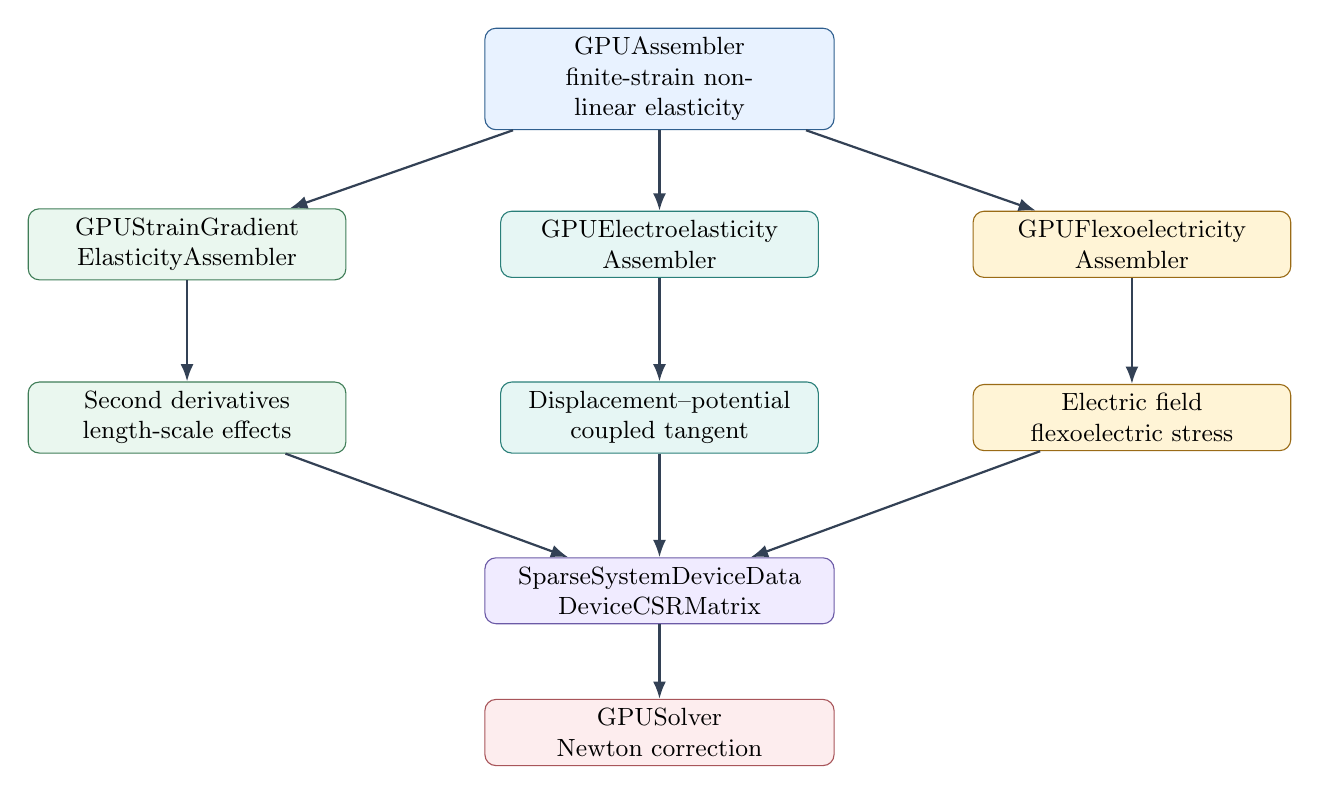
\begin{tikzpicture}[
    font=\small,
    box/.style={
        draw=sigaArrow,
        fill=white,
        rounded corners,
        align=center,
        minimum height=8mm,
        text width=42mm
    },
    smallbox/.style={
        draw=sigaArrow,
        fill=white,
        rounded corners,
        align=center,
        minimum height=8mm,
        text width=38mm
    },
    basebox/.style={box, fill=sigaBlueFill, draw=sigaBlueLine},
    strainbox/.style={smallbox, fill=sigaGreenFill, draw=sigaGreenLine},
    electrobox/.style={smallbox, fill=sigaTealFill, draw=sigaTealLine},
    flexobox/.style={smallbox, fill=sigaAmberFill, draw=sigaAmberLine},
    sparsebox/.style={box, fill=sigaPurpleFill, draw=sigaPurpleLine},
    solverbox/.style={box, fill=sigaRoseFill, draw=sigaRoseLine},
    arrow/.style={
        -{Latex[length=2.2mm]},
        thick,
        draw=sigaArrow
    }
]

\node[basebox] (base) at (0,0) {GPUAssembler\\finite-strain nonlinear elasticity};

\node[strainbox] (sg) at (-6.0,-2.1) {GPUStrainGradient\\ElasticityAssembler};
\node[electrobox] (ee) at (0,-2.1) {GPUElectroelasticity\\Assembler};
\node[flexobox] (fx) at (6.0,-2.1) {GPUFlexoelectricity\\Assembler};

\node[strainbox] (sgq) at (-6.0,-4.3) {Second derivatives\\length-scale effects};
\node[electrobox] (eeq) at (0,-4.3) {Displacement--potential\\coupled tangent};
\node[flexobox] (fxq) at (6.0,-4.3) {Electric field\\flexoelectric stress};

\node[sparsebox] (sparse) at (0,-6.5) {SparseSystemDeviceData\\DeviceCSRMatrix};
\node[solverbox] (solver) at (0,-8.3) {GPUSolver\\Newton correction};

\draw[arrow] (base) -- (sg);
\draw[arrow] (base) -- (ee);
\draw[arrow] (base) -- (fx);

\draw[arrow] (sg) -- (sgq);
\draw[arrow] (ee) -- (eeq);
\draw[arrow] (fx) -- (fxq);

\draw[arrow] (sgq) -- (sparse);
\draw[arrow] (eeq) -- (sparse);
\draw[arrow] (fxq) -- (sparse);
\draw[arrow] (sparse) -- (solver);

\end{tikzpicture}%
}
\caption{Assembler hierarchy in SIGA. The base GPU assembler provides the common nonlinear mechanics assembly infrastructure, while specialized assemblers extend the formulation to strain-gradient elasticity, electroelasticity, and flexoelectricity. All assemblers generate residual and tangent contributions in a common sparse-system format used by the Newton solver.}
\label{fig:siga_assembler_hierarchy}
\end{figure}

\subsection{Sparse Matrix Representation}

The sparse algebraic system is stored in compressed sparse row format on the device. During initialization, the sparsity pattern is constructed from the degree-of-freedom mapping and active basis connectivity. During nonlinear iterations, only the matrix values and residual entries need to be updated. This distinction between sparsity-pattern construction and value assembly is important for nonlinear problems, because the same pattern is reused over multiple Newton iterations and load steps.

SIGA uses a device CSR matrix abstraction to store row pointers, column indices, and matrix values. This representation is compatible with GPU-based solvers and can also be transferred to host-side sparse matrices when CPU solver backends are used. In the current implementation, PARDISO is the primary CPU sparse solver, while Eigen is kept as the fallback path when PARDISO support is not available. The sparse matrix layer therefore acts as an interface between the GPU assembly kernels and the available linear solver backends.

\subsection{Nonlinear Solver Layer}

The nonlinear solution procedure is implemented using a Newton iteration. At each iteration, the current solution is passed to the assembler, which computes the residual vector and tangent matrix. The linearized correction is then obtained using one of the available solver backends. When AMGX is enabled, SIGA can solve the sparse system using a GPU-based iterative solver. When AMGX is disabled or unsuitable for a particular problem, the system can be transferred to the host and solved with PARDISO as the main CPU direct solver. If PARDISO is not available in the build, SIGA falls back to Eigen-based sparse solvers. This design provides flexibility between fully GPU-oriented workflows and robust CPU-based fallback paths.

The solver layer also stores convergence information, including residual norms, update norms, iteration counts, and timing data. These quantities are useful both for controlling nonlinear simulations and for reporting performance results. In addition to standard Newton solution, the solver provides eigenvalue and stability-related functionality, which is used in buckling and instability examples.

\subsection{Post-Processing Layer}

After convergence, SIGA reconstructs physical fields from the solution vector. Displacement, stress, deformation gradient, strain-gradient quantities, electric potential, and electric field can be represented as spline-based functions. These fields are evaluated at visualization points and exported through the post-processing module. The output is written in ParaView-compatible formats, allowing the user to inspect undeformed and deformed geometries, stress distributions, electric fields, and higher-gradient quantities.

The post-processing layer is deliberately separated from the solver and assembler. This makes it possible to use the same computational core for verification studies, performance benchmarks, and application simulations while changing only the output fields required by each example.

\subsection{Design Advantages}

The main advantage of the SIGA architecture is that geometry, basis construction, physical assembly, sparse algebra, nonlinear solution, and visualization are separated into reusable modules. This design has several practical benefits. First, new physical models can reuse the same patch, basis, boundary-condition, and sparse-system infrastructure. Second, GPU kernels can be specialized for expensive model-specific operations while preserving a common solver interface. Third, the same nonlinear solver can be used across classical elasticity, strain-gradient elasticity, and coupled electro-mechanical formulations. Finally, the common post-processing interface allows different simulations to export comparable field quantities for visualization and analysis.

Overall, the architecture is intended to support extensibility and performance simultaneously. The host side handles symbolic and topological operations such as geometry construction, refinement, and degree-of-freedom mapping, while the GPU side handles the computationally intensive quadrature, residual assembly, tangent assembly, sparse matrix updates, and field recovery operations.

\section{Parallel Assembly Strategy, Multi-GPU Support, and Memory Management}
\label{sec:parallel_assembly}

The dominant computational cost in SIGA comes from repeated residual and tangent-matrix assembly during Newton iterations. This cost is especially significant for high-order isogeometric discretizations because each element contains multiple quadrature points and each quadrature point couples all active spline basis functions. SIGA therefore performs the most expensive quadrature, constitutive evaluation, and sparse assembly operations on the GPU. The assembly strategy is organized around three design principles: element-level parallelism, reuse of precomputed basis and quadrature data, and memory-aware streaming over groups of elements.

\subsection{Parallel Assembly Decomposition}

At each Newton iteration, SIGA first reconstructs the current displacement field from the solution vector and prescribed degrees of freedom. The geometry, basis values, basis derivatives, quadrature points, sparse-system metadata, and material parameters are already stored in device-side data structures. The assembly procedure then proceeds in three main phases:
\begin{enumerate}
    \item Gauss-point precomputation, where deformation measures, geometry Jacobians, integration weights, stresses, and material tangent quantities are evaluated.
    \item Tangent-matrix assembly, where element-level contributions are accumulated into the global sparse matrix.
    \item Residual-vector assembly, where internal-force and external-force contributions are accumulated into the global right-hand side.
\end{enumerate}

For a displacement discretization with \(N_e\) elements, \(N_D\) active basis functions per element, and spatial dimension \(d\), the tangent assembly can be viewed as a parallel loop over element-basis pairs
\[
    (e,i,j), \qquad
    e = 1,\ldots,N_e, \quad
    i,j = 1,\ldots,N_D .
\]
Each such task computes a local block
\[
    \mathbf{K}^{e}_{ij} \in \mathbb{R}^{d \times d},
\]
which contains all component couplings between basis functions \(N_i\) and \(N_j\). The residual assembly is similarly decomposed over element-basis pairs \((e,i)\), producing local vectors
\[
    \mathbf{R}^{e}_{i} \in \mathbb{R}^{d}.
\]
Within each CUDA block, threads iterate over quadrature points and accumulate the corresponding local matrix or residual contribution. After all quadrature contributions are accumulated, the local block is inserted into the global sparse system.

Figure~\ref{fig:parallel_assembly_decomposition} illustrates this decomposition. The important point is that SIGA does not assign an entire element matrix to a single serial thread. Instead, the element stiffness computation is broken into many block-level tasks indexed by active basis-function pairs. This strategy exposes a large amount of parallelism for high-order spline elements.

\begin{figure}[H]
\centering
\resizebox{\textwidth}{!}{%
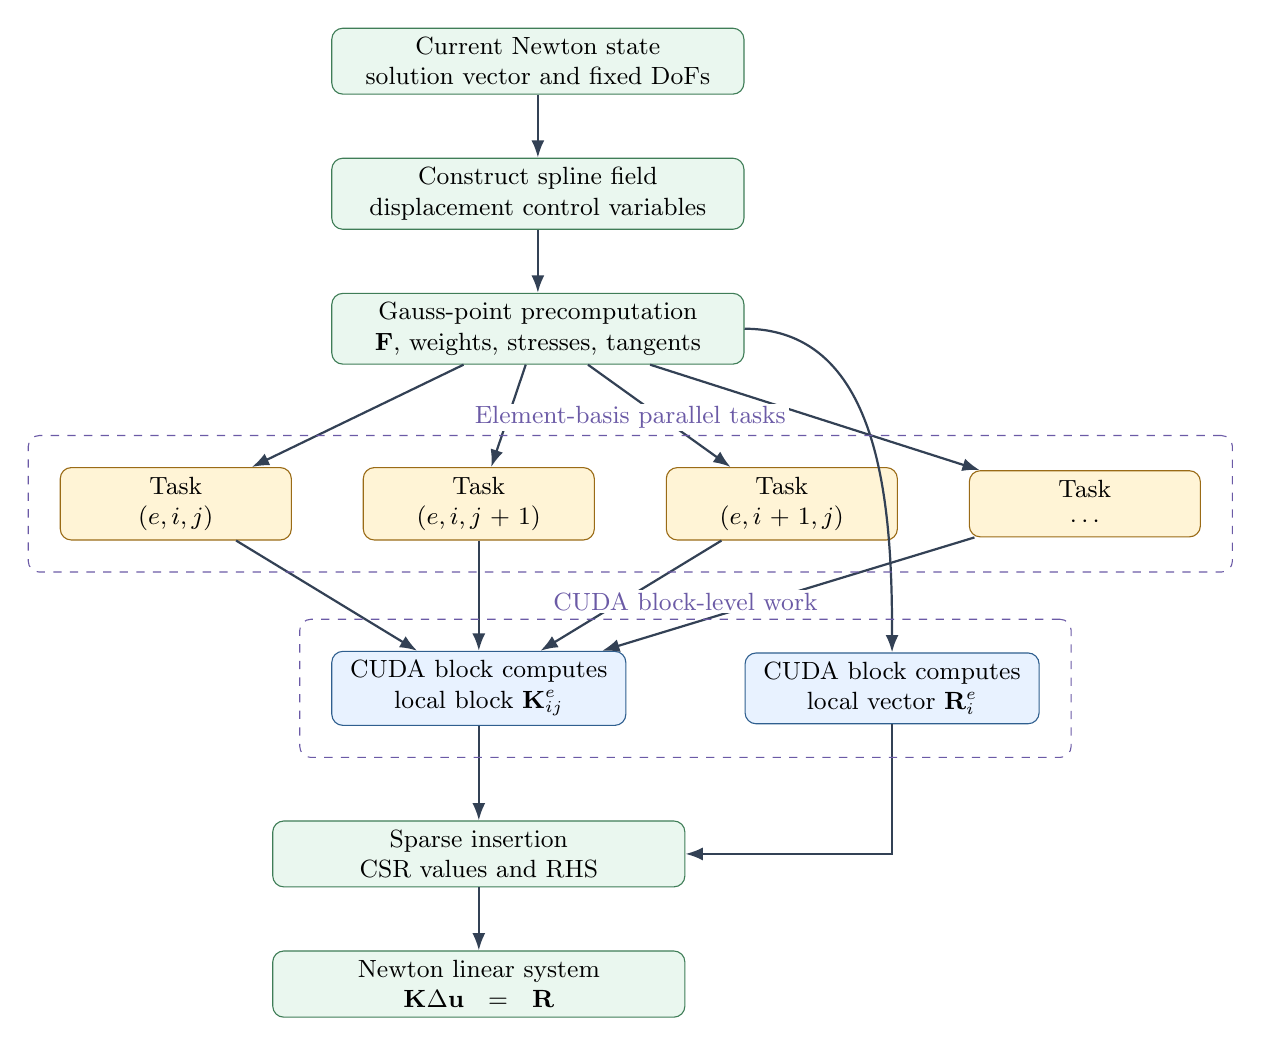
\begin{tikzpicture}[
    font=\small,
    node distance=8mm and 9mm,
    box/.style={
        draw=sigaBlueLine,
        fill=sigaBlueFill,
        rounded corners,
        align=center,
        minimum height=8mm,
        text width=35mm
    },
    widebox/.style={
        draw=sigaGreenLine,
        fill=sigaGreenFill,
        rounded corners,
        align=center,
        minimum height=8mm,
        text width=50mm
    },
    smallbox/.style={
        draw=sigaAmberLine,
        fill=sigaAmberFill,
        rounded corners,
        align=center,
        minimum height=7mm,
        text width=27mm
    },
    arrow/.style={
        -{Latex[length=2.2mm]},
        thick,
        draw=sigaArrow
    },
    group/.style={
        draw=sigaPurpleLine,
        dashed,
        rounded corners,
        inner sep=4mm
    }
]

\node[widebox] (solution) {Current Newton state\\solution vector and fixed DoFs};
\node[widebox, below=of solution] (field) {Construct spline field\\displacement control variables};
\node[widebox, below=of field] (gp) {Gauss-point precomputation\\\(\mathbf{F}\), weights, stresses, tangents};

\node[smallbox, below left=13mm and 5mm of gp] (task1) {Task\\\((e,i,j)\)};
\node[smallbox, right=of task1] (task2) {Task\\\((e,i,j+1)\)};
\node[smallbox, right=of task2] (task3) {Task\\\((e,i+1,j)\)};
\node[smallbox, right=of task3] (task4) {Task\\\(\cdots\)};

\node[box, below=14mm of task2] (localK) {CUDA block computes\\local block \(\mathbf{K}^{e}_{ij}\)};
\node[box, right=15mm of localK] (localR) {CUDA block computes\\local vector \(\mathbf{R}^{e}_{i}\)};

\node[widebox, below=12mm of localK] (insert) {Sparse insertion\\CSR values and RHS};
\node[widebox, below=of insert] (newton) {Newton linear system\\\(\mathbf{K}\Delta\mathbf{u}=\mathbf{R}\)};

\draw[arrow] (solution) -- (field);
\draw[arrow] (field) -- (gp);
\draw[arrow] (gp) -- (task1);
\draw[arrow] (gp) -- (task2);
\draw[arrow] (gp) -- (task3);
\draw[arrow] (gp) -- (task4);

\draw[arrow] (task1) -- (localK);
\draw[arrow] (task2) -- (localK);
\draw[arrow] (task3) -- (localK);
\draw[arrow] (task4) -- (localK);

\draw[arrow] (gp.east) to[out=0,in=90] (localR.north);

\draw[arrow] (localK) -- (insert);
\draw[arrow] (localR) |- (insert);
\draw[arrow] (insert) -- (newton);

\node[group, fit=(task1)(task2)(task3)(task4)] (taskgroup) {};
\node[font=\small, text=sigaPurpleLine, fill=white, inner sep=1pt]
    at ($(taskgroup.north)+(0,0.22)$) {Element-basis parallel tasks};
\node[group, fit=(localK)(localR)] (workgroup) {};
\node[font=\small, text=sigaPurpleLine, fill=white, inner sep=1pt]
    at ($(workgroup.north)+(0,0.22)$) {CUDA block-level work};

\end{tikzpicture}%
}
\caption{Parallel decomposition of SIGA's GPU assembly. The tangent matrix is decomposed into element-basis pair tasks \((e,i,j)\), while the residual vector is decomposed into element-basis tasks \((e,i)\). Each CUDA block accumulates quadrature-point contributions for a small local block before inserting the result into the global sparse system.}
\label{fig:parallel_assembly_decomposition}
\end{figure}
\FloatBarrier

The same decomposition is used for higher-gradient formulations, but with additional Gauss-point data. In strain-gradient elasticity, for example, the local tangent block contains contributions from both first-gradient and second-gradient terms. The block-level computation uses precomputed geometry inverses, weights, geometry Hessians, stress-like quantities, and material tangent blocks. The local tangent contribution includes contractions of the form
\[
    \mathbf{B}_i^{T}
    \frac{\partial \mathbf{P}_1}{\partial \mathbf{F}}
    \mathbf{B}_j,
    \qquad
    \mathbf{B}_i^{T}
    \frac{\partial \mathbf{P}_1}{\partial \nabla \mathbf{F}}
    \mathbf{D}_j,
    \qquad
    \mathbf{D}_i^{T}
    \frac{\partial \mathbf{P}_2}{\partial \nabla \mathbf{F}}
    \mathbf{D}_j ,
\]
where \(\mathbf{B}\) denotes the first-gradient operator and \(\mathbf{D}\) denotes the second-gradient operator. This structure is well suited to IGA because the higher continuity of spline basis functions allows second derivatives to be evaluated inside patches.

\subsection{Sparse Assembly and Fixed-Degree-of-Freedom Treatment}

SIGA stores the global tangent matrix in compressed sparse row format. The sparsity pattern is built from the active basis connectivity and degree-of-freedom mapping, while the matrix values are updated during each Newton iteration. During insertion, each local contribution is mapped from patch-local active basis indices to global row and column indices. Free degrees of freedom contribute directly to the CSR matrix. Contributions associated with eliminated fixed degrees of freedom are redirected to the right-hand side, which allows Dirichlet constraints to be handled consistently inside the same assembly path.

This design avoids forming dense element matrices on the host. Instead, element-level contributions are accumulated directly into device-side sparse data structures. The sparse assembly layer therefore acts as the interface between local quadrature computations and the global Newton system.

\subsection{Streaming Assembly}

For very large problems, storing all temporary Gauss-point data for the entire domain can exceed available GPU memory. SIGA addresses this issue through streaming assembly. Instead of assembling the whole domain in one pass, the element range is divided into chunks. Each chunk contains a contiguous set of elements, the associated Gauss points, and the corresponding local sparse row window. The assembly kernels are then applied chunk by chunk.

For each chunk, SIGA performs the following operations:
\begin{enumerate}
    \item determine the element range and Gauss-point range;
    \item determine the affected sparse row range;
    \item allocate or reuse temporary Gauss-point buffers;
    \item evaluate Gauss-point quantities for the chunk;
    \item assemble the chunk-local tangent and residual;
    \item accumulate the chunk contribution into the global CSR matrix and RHS vector.
\end{enumerate}

Figure~\ref{fig:streaming_assembly} shows one streaming step. The full element set is kept as a host-side chunk schedule, but the GPU temporary-memory window contains only the active chunk, its Gauss-point data, and the affected sparse row window. After that chunk is accumulated into the global CSR matrix and RHS vector, the temporary buffers are released or reused for the next chunk. The same code path can run on a single GPU or across multiple GPUs. When only one GPU is used, streaming mainly reduces peak memory usage. When multiple GPUs are used, the chunks are distributed across devices.

\begin{figure}[H]
\centering
\resizebox{\textwidth}{!}{%
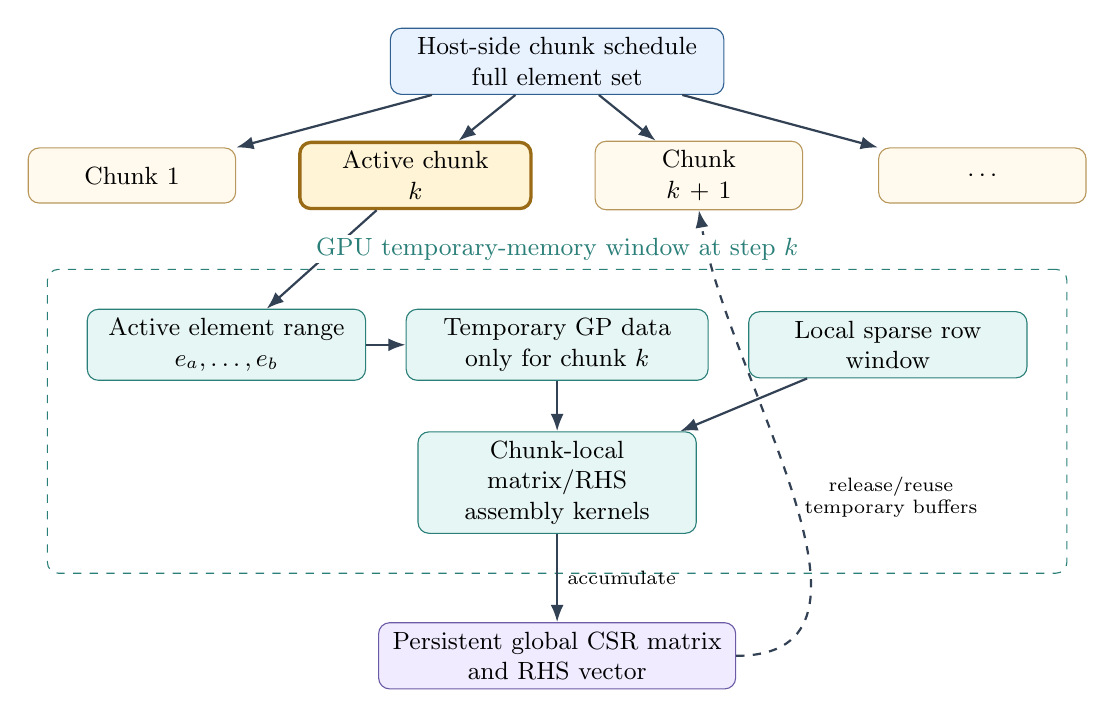
\begin{tikzpicture}[
    font=\small,
    hostbox/.style={
        draw=sigaBlueLine,
        fill=sigaBlueFill,
        rounded corners,
        align=center,
        minimum height=8mm,
        text width=40mm
    },
    inactivechunk/.style={
        draw=sigaAmberLine!70,
        fill=sigaAmberFill!45,
        rounded corners,
        align=center,
        minimum height=7mm,
        text width=24mm
    },
    activechunk/.style={
        draw=sigaAmberLine,
        fill=sigaAmberFill,
        very thick,
        rounded corners,
        align=center,
        minimum height=7mm,
        text width=27mm
    },
    workbox/.style={
        draw=sigaTealLine,
        fill=sigaTealFill,
        rounded corners,
        align=center,
        minimum height=8mm,
        text width=33mm
    },
    gpbox/.style={
        draw=sigaTealLine,
        fill=sigaTealFill,
        rounded corners,
        align=center,
        minimum height=8mm,
        text width=36mm
    },
    persistentbox/.style={
        draw=sigaPurpleLine,
        fill=sigaPurpleFill,
        rounded corners,
        align=center,
        minimum height=8mm,
        text width=43mm
    },
    arrow/.style={
        -{Latex[length=2.2mm]},
        thick,
        draw=sigaArrow
    },
    dashedarrow/.style={
        -{Latex[length=2.2mm]},
        thick,
        dashed,
        draw=sigaArrow
    },
    groupbox/.style={
        draw=sigaTealLine,
        dashed,
        rounded corners,
        inner xsep=5mm,
        inner ysep=5mm
    }
]

\node[hostbox] (schedule) at (0,0) {Host-side chunk schedule\\full element set};

\node[inactivechunk] (c1) at (-5.4,-1.45) {Chunk 1};
\node[activechunk] (ck) at (-1.8,-1.45) {Active chunk\\\(k\)};
\node[inactivechunk] (cnext) at (1.8,-1.45) {Chunk\\\(k+1\)};
\node[inactivechunk] (cdots) at (5.4,-1.45) {\(\cdots\)};

\node[workbox] (active) at (-4.2,-3.6) {Active element range\\\(e_a,\ldots,e_b\)};
\node[gpbox] (gp) at (0,-3.6) {Temporary GP data\\only for chunk \(k\)};
\node[workbox] (rowwin) at (4.2,-3.6) {Local sparse row\\window};
\node[workbox] (assemble) at (0,-5.35) {Chunk-local matrix/RHS\\assembly kernels};

\node[groupbox, fit=(active)(gp)(rowwin)(assemble)] (gpuwindow) {};

\node[persistentbox] (global) at (0,-7.55) {Persistent global CSR matrix\\and RHS vector};

\draw[arrow] (schedule) -- (c1);
\draw[arrow] (schedule) -- (ck);
\draw[arrow] (schedule) -- (cnext);
\draw[arrow] (schedule) -- (cdots);

\draw[arrow] (ck) -- (active);
\draw[arrow] (active) -- (gp);
\draw[arrow] (gp) -- (assemble);
\draw[arrow] (rowwin) -- (assemble);
\draw[arrow] (assemble) -- node[right, font=\scriptsize] {accumulate} (global);

\draw[dashedarrow] (global.east) to[out=0,in=-80]
    node[right, font=\scriptsize, align=center] {release/reuse\\temporary buffers}
    (cnext.south);
\node[font=\small, text=sigaTealLine, fill=white, inner xsep=2pt, inner ysep=1pt]
    at ($(gpuwindow.north)+(0,0.25)$) {GPU temporary-memory window at step \(k\)};

\end{tikzpicture}%
}
\caption{Streaming assembly strategy. The full element set is divided into a host-side chunk schedule, but only the active chunk \(k\), its Gauss-point data, and its sparse row window occupy temporary GPU buffers at a given streaming step. After the chunk-local matrix and residual are accumulated into the persistent global CSR matrix and RHS vector, the temporary buffers are released or reused for the next chunk.}
\label{fig:streaming_assembly}
\end{figure}
\FloatBarrier

\subsection{Multi-GPU Assembly}

Multi-GPU assembly in SIGA extends the streaming strategy by distributing chunks over all usable CUDA devices. SIGA first identifies the primary CUDA device and then scans the visible devices. A secondary device is used only if peer access is available in both directions between the primary device and the secondary device. Peer access is enabled before the assembly begins. This check avoids assigning work to GPUs that cannot exchange data efficiently with the primary device.

The primary GPU stores the global CSR matrix and RHS vector. Secondary GPUs receive replicated static input data, such as geometry, basis, Gauss-point tables, material data, and sparse metadata. During each Newton iteration, dynamic data such as displacement control points and fixed degrees of freedom are refreshed. Each secondary GPU assembles into a local sparse output buffer, which contains only the matrix-value and RHS entries associated with its assigned sparse row window. After each round of chunk assembly, the secondary output buffers are reduced into the global CSR matrix and RHS on the primary GPU.

Figure~\ref{fig:multigpu_assembly} summarizes the multi-GPU data flow.

\begin{figure}[H]
\centering
\resizebox{\textwidth}{!}{%
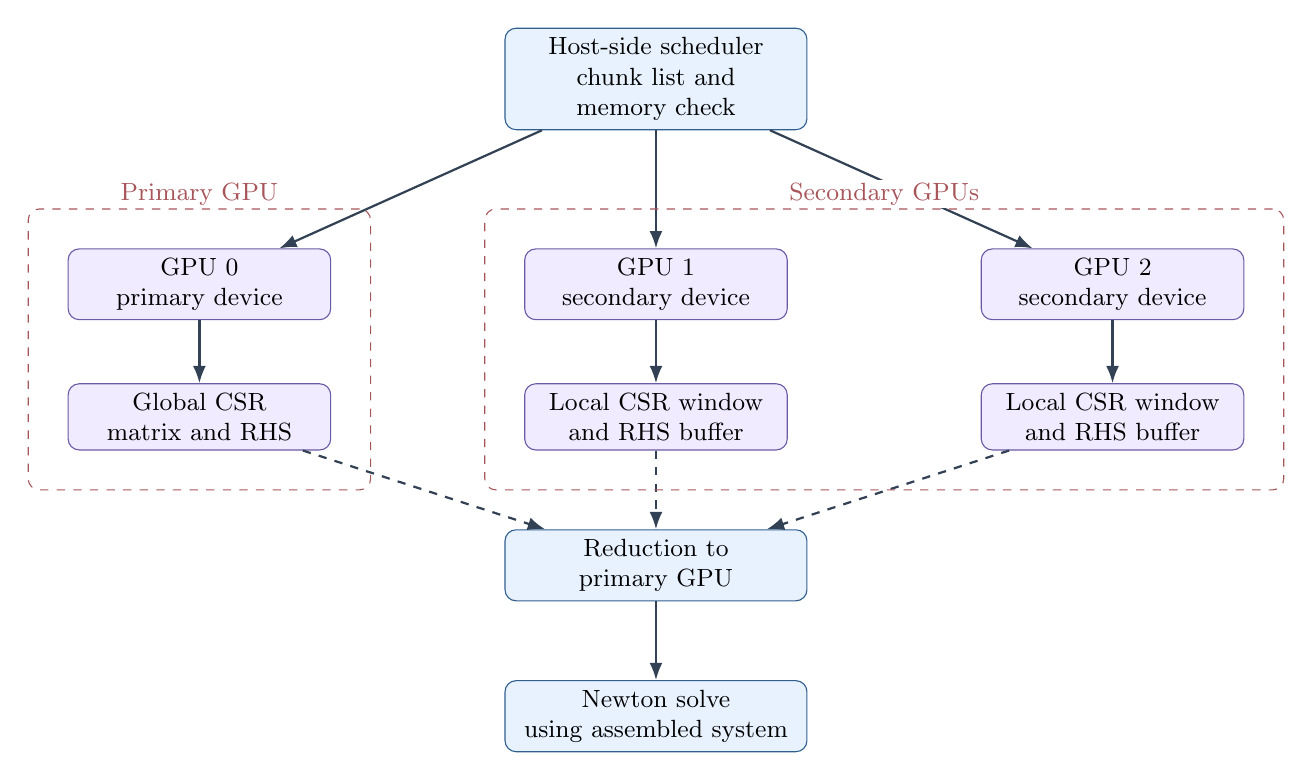
\begin{tikzpicture}[
    font=\small,
    node distance=8mm and 9mm,
    box/.style={
        draw=sigaBlueLine,
        fill=sigaBlueFill,
        rounded corners,
        align=center,
        minimum height=8mm,
        text width=36mm
    },
    smallbox/.style={
        draw=sigaPurpleLine,
        fill=sigaPurpleFill,
        rounded corners,
        align=center,
        minimum height=7mm,
        text width=31mm
    },
    arrow/.style={
        -{Latex[length=2.2mm]},
        thick,
        draw=sigaArrow
    },
    dashedarrow/.style={
        -{Latex[length=2.2mm]},
        thick,
        dashed,
        draw=sigaArrow
    },
    group/.style={
        draw=sigaRoseLine,
        dashed,
        rounded corners,
        inner sep=5mm
    }
]

\node[box] (host) {Host-side scheduler\\chunk list and memory check};

\node[smallbox, below left=15mm and 22mm of host] (gpu0) {GPU 0\\primary device};
\node[smallbox, below=15mm of host] (gpu1) {GPU 1\\secondary device};
\node[smallbox, below right=15mm and 22mm of host] (gpu2) {GPU 2\\secondary device};

\node[smallbox, below=8mm of gpu0] (global) {Global CSR\\matrix and RHS};
\node[smallbox, below=8mm of gpu1] (buf1) {Local CSR window\\and RHS buffer};
\node[smallbox, below=8mm of gpu2] (buf2) {Local CSR window\\and RHS buffer};

\node[box, below=10mm of buf1] (reduce) {Reduction to\\primary GPU};

\node[box, below=10mm of reduce] (newton) {Newton solve\\using assembled system};

\draw[arrow] (host) -- (gpu0);
\draw[arrow] (host) -- (gpu1);
\draw[arrow] (host) -- (gpu2);

\draw[arrow] (gpu0) -- (global);
\draw[arrow] (gpu1) -- (buf1);
\draw[arrow] (gpu2) -- (buf2);

\draw[dashedarrow] (global) -- (reduce);
\draw[dashedarrow] (buf1) -- (reduce);
\draw[dashedarrow] (buf2) -- (reduce);

\draw[arrow] (reduce) -- (newton);

\node[group, fit=(gpu0)(global)] (primarygroup) {};
\node[group, fit=(gpu1)(gpu2)(buf1)(buf2)] (secondarygroup) {};
\node[font=\small, text=sigaRoseLine, fill=white, inner xsep=2pt, inner ysep=1pt]
    at ($(primarygroup.north)+(0,0.18)$) {Primary GPU};
\node[font=\small, text=sigaRoseLine, fill=white, inner xsep=2pt, inner ysep=1pt]
    at ($(secondarygroup.north)+(0,0.18)$) {Secondary GPUs};

\end{tikzpicture}%
}
\caption{Multi-GPU assembly in SIGA. The primary GPU owns the global sparse system. Secondary GPUs assemble assigned chunks into local sparse output buffers. After each assembly round, local matrix values and residual entries are reduced into the primary CSR matrix and RHS vector.}
\label{fig:multigpu_assembly}
\end{figure}
\FloatBarrier

The chunk distribution is round-robin. If \(n_g\) usable GPUs are available, chunk \(k\) is assigned to device
\[
    g(k) = k \bmod n_g .
\]
This simple policy keeps the implementation robust and avoids complicated load-balancing overhead. Since the chunks are generated with a bounded maximum number of elements, the amount of work per chunk is approximately controlled by the user-specified or automatically reduced chunk size.

Within each round, SIGA launches chunk work on all devices that have an available chunk. The implementation uses one host thread per active device in a round. Each host thread sets its CUDA device, launches the Gauss-point precomputation, matrix assembly, and RHS assembly kernels for the assigned chunk, and synchronizes the device. After all device threads complete, the primary device performs the reduction of secondary sparse output buffers.

\subsection{Memory-Aware Chunk Sizing}

The streaming and multi-GPU assembly path is memory-aware. SIGA estimates the amount of temporary memory required on each device before launching the assembly. The estimate includes:
\begin{itemize}
    \item local matrix-value output buffer;
    \item local RHS output buffer;
    \item material-parameter array;
    \item Gauss-point temporary data;
    \item sparse metadata and local CSR row window;
    \item replicated static input data;
    \item replicated fixed-degree-of-freedom data.
\end{itemize}

Let \(M_g\) denote the currently free memory on GPU \(g\), and let \(\eta\in(0,1]\) denote the memory safety fraction. SIGA requires
\[
    M^{\mathrm{req}}_g \leq \eta M_g .
\]
If the requested chunk size violates this inequality, SIGA automatically reduces the maximum number of elements per chunk and rebuilds the schedule. This procedure is repeated until the schedule fits within the memory target or until even a one-element chunk cannot fit. The safety fraction is controlled by the environment variable
\[
    \texttt{SIGA\_GPU\_MEMORY\_FRACTION}.
\]
The initial chunk size can be specified using
\[
    \texttt{SIGA\_GPU\_CHUNK\_ELEMENTS}.
\]
If no chunk size is specified, SIGA starts from a one-shot partition in which the elements are divided approximately evenly among the usable assembly devices.

Figure~\ref{fig:memory_management} illustrates the memory-management loop.

\begin{figure}[H]
\centering
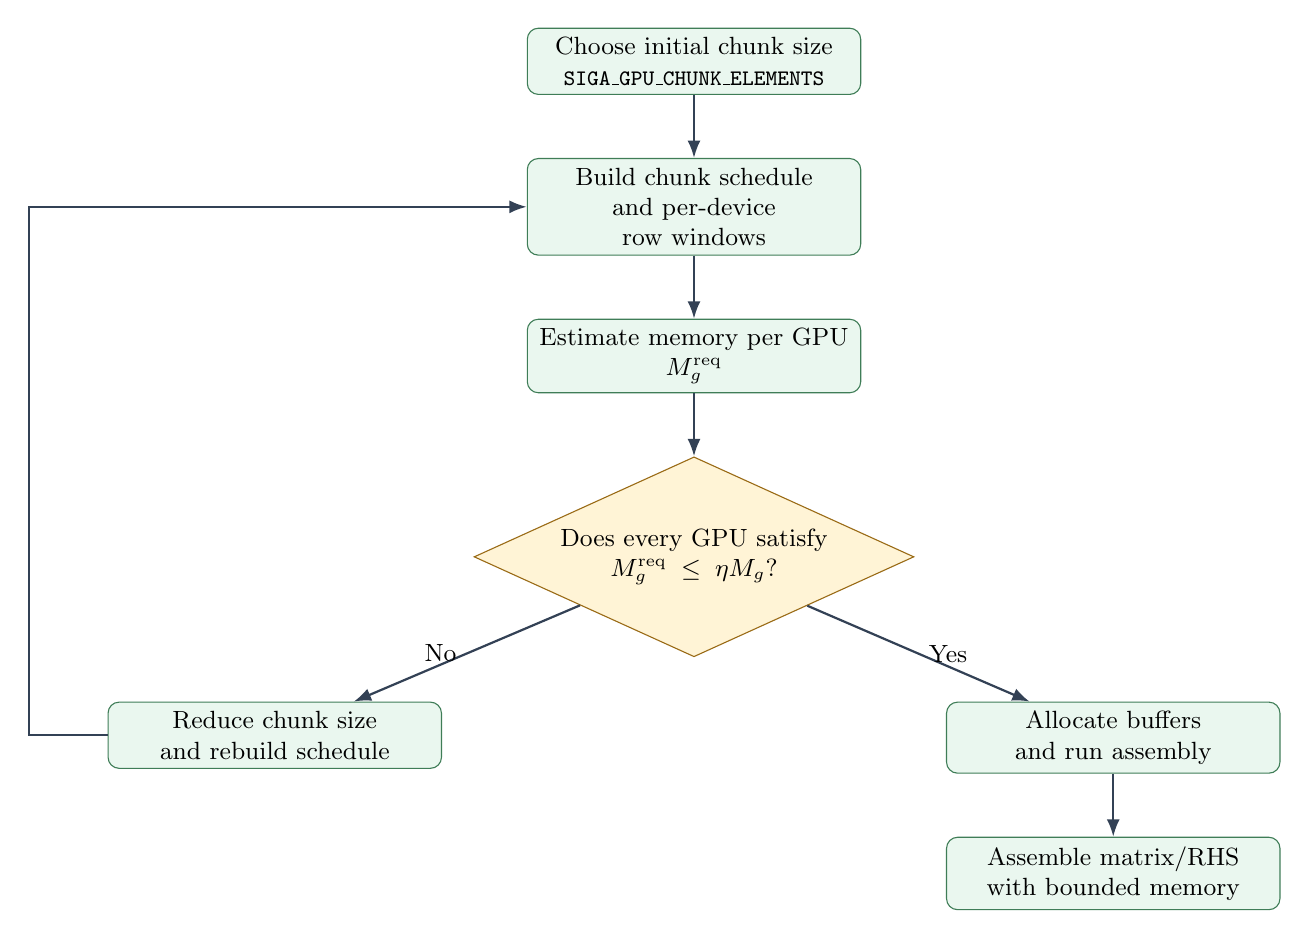
\begin{tikzpicture}[
    font=\small,
    node distance=8mm and 10mm,
    box/.style={
        draw=sigaGreenLine,
        fill=sigaGreenFill,
        rounded corners,
        align=center,
        minimum height=8mm,
        text width=40mm
    },
    decision/.style={
        draw=sigaAmberLine,
        fill=sigaAmberFill,
        diamond,
        aspect=2.2,
        align=center,
        inner sep=1mm,
        text width=34mm
    },
    arrow/.style={
        -{Latex[length=2.2mm]},
        thick,
        draw=sigaArrow
    }
]

\node[box] (start) {Choose initial chunk size\\{\footnotesize\(\texttt{SIGA\_GPU\_CHUNK\_ELEMENTS}\)}};
\node[box, below=of start] (schedule) {Build chunk schedule\\and per-device row windows};
\node[box, below=of schedule] (estimate) {Estimate memory per GPU\\\(M_g^{\mathrm{req}}\)};
\node[decision, below=of estimate] (fit) {Does every GPU satisfy\\\(M_g^{\mathrm{req}} \leq \eta M_g\)?};
\node[box, below left=12mm and 18mm of fit] (reduce) {Reduce chunk size\\and rebuild schedule};
\node[box, below right=12mm and 18mm of fit] (run) {Allocate buffers\\and run assembly};
\node[box, below=of run] (finish) {Assemble matrix/RHS\\with bounded memory};

\draw[arrow] (start) -- (schedule);
\draw[arrow] (schedule) -- (estimate);
\draw[arrow] (estimate) -- (fit);

\draw[arrow] (fit) -- node[left] {No} (reduce);
\draw[arrow] (reduce.west) -- ++(-10mm,0) |- (schedule.west);

\draw[arrow] (fit) -- node[right] {Yes} (run);
\draw[arrow] (run) -- (finish);

\end{tikzpicture}
\caption{Memory-aware chunk-size selection. SIGA estimates the required temporary memory on each GPU and compares it with a safety fraction of the currently available memory. If the schedule does not fit, the element chunk size is reduced and the schedule is rebuilt.}
\label{fig:memory_management}
\end{figure}
\FloatBarrier

The memory-management strategy is particularly important for higher-order IGA. For a degree-\(p\) tensor-product basis in \(d\) dimensions, the number of active basis functions per element scales approximately as
\[
    N_D \sim (p+1)^d .
\]
The local tangent work therefore scales with \(N_D^2\), and the temporary quadrature data also increase with the number of Gauss points and derivative quantities stored per point. In higher-gradient problems, the memory footprint is even larger because the formulation requires second derivatives, geometry Hessians, and additional constitutive tangent blocks. Streaming assembly allows SIGA to handle these cases without requiring all temporary element and Gauss-point data to be resident simultaneously.

\subsection{Configurable Assembly Modes}

The assembly behavior can be controlled at runtime without recompilation. The most relevant environment variables are:
\begin{itemize}
    \item \texttt{SIGA\_MULTIGPU\_ASSEMBLY}: enables multi-GPU assembly.
    \item \texttt{SIGA\_GPU\_STREAMING\_ASSEMBLY}: enables streaming assembly. By default, streaming is enabled when multi-GPU assembly is enabled.
    \item \texttt{SIGA\_GPU\_CHUNK\_ELEMENTS}: sets the requested maximum number of elements per chunk.
    \item \texttt{SIGA\_GPU\_MEMORY\_FRACTION}: sets the safety fraction used in memory fitting.
    \item \texttt{SIGA\_GPU\_REPLICATE\_INPUTS}: controls whether secondary GPUs receive replicated geometry, basis, and quadrature input data.
    \item \texttt{SIGA\_GPU\_LOCAL\_CSR\_ASSEMBLY}: controls whether secondary GPUs assemble into local CSR row windows.
    \item \texttt{SIGA\_GPU\_MATRIX\_TIMING}: enables detailed timing output for assembly phases.
    \item \texttt{SIGA\_GPU\_MEMORY\_REPORT}: enables memory diagnostics for assembly buffers.
\end{itemize}

These options make it possible to use the same executable in several modes. For small problems, a one-shot single-GPU assembly may be sufficient. For large problems that exceed the memory available for temporary Gauss-point data, streaming can be enabled on one GPU. For still larger problems or for machines with multiple peer-accessible GPUs, multi-GPU streaming distributes chunks across devices and reduces their local sparse outputs to the primary device.

\subsection{Discussion}

The proposed parallel assembly strategy reflects the structure of isogeometric discretizations. High-order spline elements produce expensive element-level operations because many active basis functions interact over each element. SIGA exposes this work by parallelizing over elements, active basis pairs, quadrature points, and field components. Temporary Gauss-point quantities are reused between matrix and residual assembly, while the global sparse system remains in CSR format throughout the Newton iteration.

The multi-GPU implementation follows a primary-secondary model. The primary GPU owns the global sparse matrix and residual vector, while secondary GPUs assemble assigned chunks into local output buffers. This design avoids concurrent writes from multiple devices into the same global CSR array and gives a clear reduction point after each chunk round. The memory-aware chunking mechanism further ensures that the assembly can be adapted to different GPU memory capacities by reducing the number of elements processed in each chunk.

Overall, SIGA's assembly strategy is designed to balance three competing requirements: high parallel throughput, compatibility with sparse Newton solvers, and robustness for large high-order simulations whose temporary memory requirements may exceed the capacity of a single GPU.

\section{Smallest Eigenpair Computation for Stability Analysis}
\label{sec:smallest_eigenpair}

In nonlinear mechanics simulations, loss of stability is commonly associated with the loss of positive definiteness or near-singularity of the tangent stiffness matrix. SIGA therefore provides routines for computing the critical eigenpair of the assembled tangent operator. The implementation supports two cases: a single-field displacement formulation and a coupled displacement--electric-potential formulation. In both cases, the objective is not to solve a dynamic modal problem with a mass matrix, but rather to identify the critical static tangent eigenmode associated with material or structural instability.

\subsection{Single Displacement Field Formulation}

For the pure mechanical formulation, the unknown vector contains only displacement degrees of freedom,
\[
    \mathbf{q} = \mathbf{u}.
\]
After the current Newton state has been reconstructed, SIGA assembles the tangent matrix
\[
    \mathbf{K}_{uu} =
    \frac{\partial \mathbf{R}_{u}}{\partial \mathbf{u}},
\]
where \(\mathbf{R}_{u}\) denotes the mechanical residual. The critical eigenpair is obtained from
\[
    \mathbf{K}_{uu}\boldsymbol{\psi}
    =
    \lambda \boldsymbol{\psi}.
\]
Here, \(\lambda\) is the tangent eigenvalue and \(\boldsymbol{\psi}\) is the corresponding displacement eigenmode. A vanishing or negative value of \(\lambda\) indicates loss of local stability of the current equilibrium path.

SIGA computes this eigenpair using an inverse iteration. Starting from a normalized vector \(\boldsymbol{x}_0\), the algorithm repeatedly solves
\[
    \mathbf{K}_{uu}\boldsymbol{y}_{k}
    =
    \boldsymbol{x}_{k},
\]
then normalizes
\[
    \boldsymbol{x}_{k+1}
    =
    \frac{\boldsymbol{y}_{k}}{\|\boldsymbol{y}_{k}\|}.
\]
The inverse eigenvalue is estimated from
\[
    \mu_k
    =
    \boldsymbol{x}_{k}^{T}\boldsymbol{y}_{k},
\]
and the tangent eigenvalue is approximated by
\[
    \lambda_k
    =
    \frac{1}{\mu_k}.
\]
The iteration stops when the change in \(\lambda_k\) is sufficiently small. After convergence, SIGA recomputes the eigenvalue using the Rayleigh quotient
\[
    \lambda
    =
    \boldsymbol{x}^{T}\mathbf{K}_{uu}\boldsymbol{x},
\]
and returns \(\boldsymbol{x}\) as the displacement eigenvector.

Figure~\ref{fig:single_field_eigenpair} summarizes the single-field computation.

\begin{figure}[H]
\centering
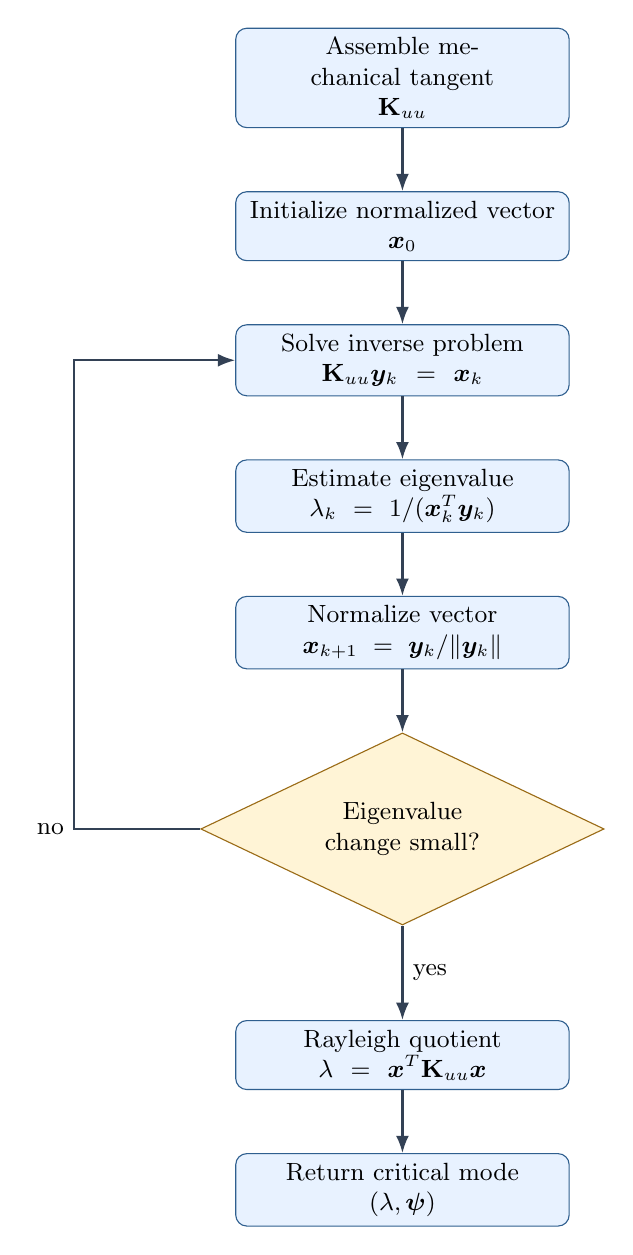
\begin{tikzpicture}[
    font=\small,
    node distance=8mm and 12mm,
    box/.style={
        draw=sigaBlueLine,
        fill=sigaBlueFill,
        rounded corners,
        align=center,
        minimum height=8mm,
        text width=40mm
    },
    decision/.style={
        draw=sigaAmberLine,
        fill=sigaAmberFill,
        diamond,
        aspect=2.1,
        align=center,
        inner sep=1mm,
        text width=31mm
    },
    arrow/.style={
        -{Latex[length=2.2mm]},
        thick,
        draw=sigaArrow
    }
]

\node[box] (assemble) {Assemble mechanical tangent\\\(\mathbf{K}_{uu}\)};
\node[box, below=of assemble] (init) {Initialize normalized vector\\\(\boldsymbol{x}_0\)};
\node[box, below=of init] (solve) {Solve inverse problem\\\(\mathbf{K}_{uu}\boldsymbol{y}_k=\boldsymbol{x}_k\)};
\node[box, below=of solve] (estimate) {Estimate eigenvalue\\\(\lambda_k = 1/(\boldsymbol{x}_k^T\boldsymbol{y}_k)\)};
\node[box, below=of estimate] (normalize) {Normalize vector\\\(\boldsymbol{x}_{k+1}=\boldsymbol{y}_k/\|\boldsymbol{y}_k\|\)};
\node[decision, below=of normalize] (conv) {Eigenvalue\\change small?};
\node[box, below=12mm of conv] (rq) {Rayleigh quotient\\\(\lambda=\boldsymbol{x}^T\mathbf{K}_{uu}\boldsymbol{x}\)};
\node[box, below=of rq] (output) {Return critical mode\\\((\lambda,\boldsymbol{\psi})\)};

\draw[arrow] (assemble) -- (init);
\draw[arrow] (init) -- (solve);
\draw[arrow] (solve) -- (estimate);
\draw[arrow] (estimate) -- (normalize);
\draw[arrow] (normalize) -- (conv);
\draw[arrow] (conv) -- node[right] {yes} (rq);
\draw[arrow] (rq) -- (output);

\draw[arrow] (conv.west) -- ++(-16mm,0) node[left] {no} |- (solve.west);

\end{tikzpicture}
\caption{Smallest critical eigenpair computation for the single displacement-field formulation. SIGA uses inverse iteration on the assembled mechanical tangent matrix and evaluates the final eigenvalue by a Rayleigh quotient.}
\label{fig:single_field_eigenpair}
\end{figure}
\FloatBarrier

The linear solve inside the inverse iteration can use different backends. When AMGX support is enabled, the tangent matrix is uploaded in CSR format and the inverse-iteration solve is performed using the AMGX solver. If AMGX fails to converge, SIGA falls back to a CPU sparse direct solve. When AMGX is not enabled, the matrix is converted to a host-side sparse matrix and solved using either PARDISO, when available, or Eigen's sparse solver backend. In incremental simulations, the previously computed eigenvector can be reused as the initial vector, which reduces the number of inverse-iteration steps needed after small load increments.

\subsection{Coupled Displacement--Electric-Potential Formulation}

For electroelastic and flexoelectric problems, the unknown vector contains both displacement and electric-potential degrees of freedom,
\[
    \mathbf{q}
    =
    \begin{bmatrix}
    \mathbf{u} \\
    \boldsymbol{\phi}
    \end{bmatrix}.
\]
The linearized coupled tangent system has the block form
\[
    \mathbf{H}
    =
    \begin{bmatrix}
    \mathbf{H}_{uu} & \mathbf{H}_{u\phi} \\
    \mathbf{H}_{\phi u} & \mathbf{H}_{\phi\phi}
    \end{bmatrix},
\]
where \(\mathbf{H}_{uu}\) is the mechanical tangent block, \(\mathbf{H}_{\phi\phi}\) is the electric-potential block, and the off-diagonal blocks describe electro-mechanical coupling.

For stability analysis, SIGA computes a condensed mechanical eigenpair. The electric-potential increment is eliminated from the coupled system by assuming that the electric field remains equilibrated with respect to a given mechanical perturbation. From the second block row,
\[
    \mathbf{H}_{\phi u}\Delta \mathbf{u}
    +
    \mathbf{H}_{\phi\phi}\Delta \boldsymbol{\phi}
    =
    \mathbf{0},
\]
we obtain
\[
    \Delta \boldsymbol{\phi}
    =
    -
    \mathbf{H}_{\phi\phi}^{-1}
    \mathbf{H}_{\phi u}\Delta \mathbf{u}.
\]
Substituting this expression into the first block row gives the condensed mechanical tangent
\[
    \widehat{\mathbf{H}}_{uu}
    =
    \mathbf{H}_{uu}
    -
    \mathbf{H}_{u\phi}
    \mathbf{H}_{\phi\phi}^{-1}
    \mathbf{H}_{\phi u}.
\]
The critical coupled stability problem is then written as
\[
    \widehat{\mathbf{H}}_{uu}\boldsymbol{\psi}_{u}
    =
    \lambda \boldsymbol{\psi}_{u}.
\]
After the mechanical eigenvector \(\boldsymbol{\psi}_{u}\) is found, the associated electric-potential eigenvector is recovered by
\[
    \boldsymbol{\psi}_{\phi}
    =
    -
    \mathbf{H}_{\phi\phi}^{-1}
    \mathbf{H}_{\phi u}
    \boldsymbol{\psi}_{u}.
\]

SIGA does not need to explicitly form \(\widehat{\mathbf{H}}_{uu}^{-1}\) for the inverse iteration. Instead, at each inverse-iteration step, it solves the full coupled system
\[
    \begin{bmatrix}
    \mathbf{H}_{uu} & \mathbf{H}_{u\phi} \\
    \mathbf{H}_{\phi u} & \mathbf{H}_{\phi\phi}
    \end{bmatrix}
    \begin{bmatrix}
    \boldsymbol{y}_{u,k} \\
    \boldsymbol{y}_{\phi,k}
    \end{bmatrix}
    =
    \begin{bmatrix}
    \boldsymbol{x}_{u,k} \\
    \mathbf{0}
    \end{bmatrix}.
\]
The displacement part \(\boldsymbol{y}_{u,k}\) is equivalent to applying the inverse of the condensed operator,
\[
    \boldsymbol{y}_{u,k}
    =
    \widehat{\mathbf{H}}_{uu}^{-1}
    \boldsymbol{x}_{u,k}.
\]
The mechanical vector is then normalized,
\[
    \boldsymbol{x}_{u,k+1}
    =
    \frac{\boldsymbol{y}_{u,k}}{\|\boldsymbol{y}_{u,k}\|},
\]
and the eigenvalue is estimated as
\[
    \lambda_k
    =
    \frac{1}{\boldsymbol{x}_{u,k}^{T}\boldsymbol{y}_{u,k}}.
\]
After convergence, SIGA evaluates the final condensed Rayleigh quotient,
\[
    \lambda
    =
    \boldsymbol{x}_{u}^{T}
    \widehat{\mathbf{H}}_{uu}
    \boldsymbol{x}_{u},
\]
and recovers the electric-potential eigenvector by back-substitution.

Figure~\ref{fig:coupled_condensed_eigenpair} illustrates the coupled-field procedure.

\begin{figure}[H]
\centering
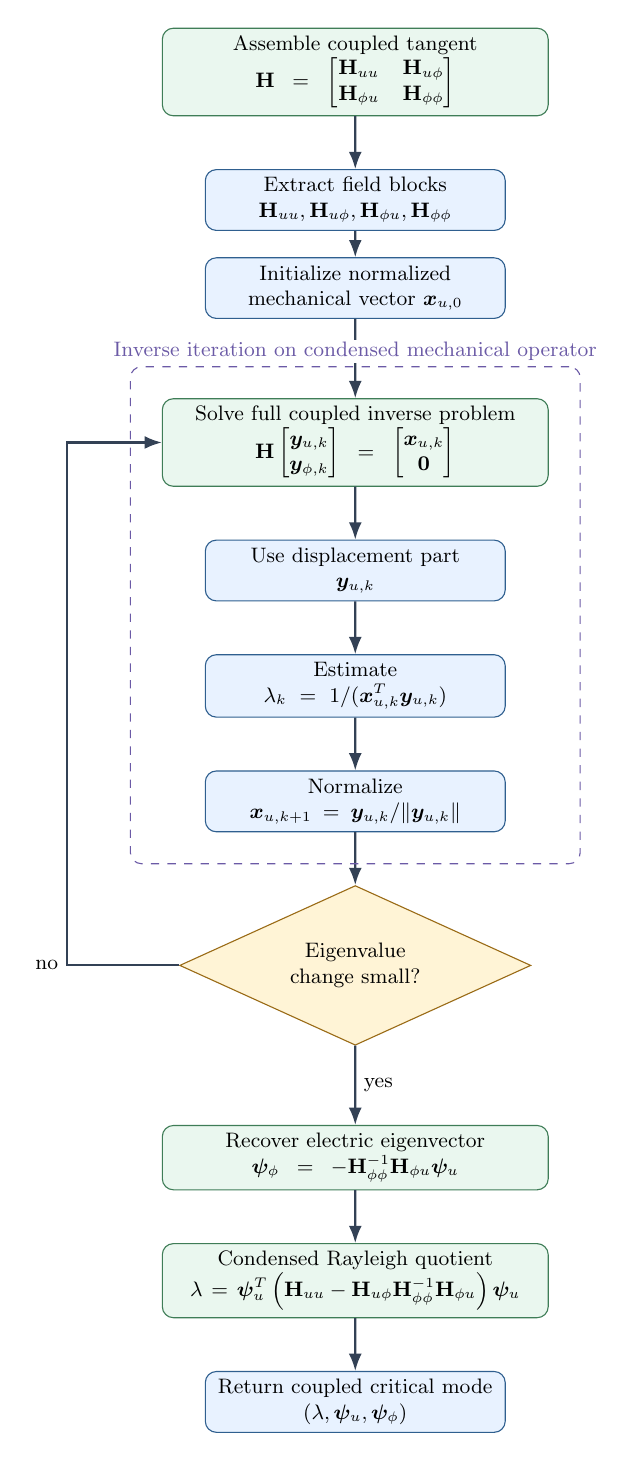
\begin{tikzpicture}[
    font=\small,
    scale=0.84,
    transform shape,
    node distance=8mm and 12mm,
    box/.style={
        draw=sigaBlueLine,
        fill=sigaBlueFill,
        rounded corners,
        align=center,
        minimum height=8mm,
        text width=43mm
    },
    widebox/.style={
        draw=sigaGreenLine,
        fill=sigaGreenFill,
        rounded corners,
        align=center,
        minimum height=8mm,
        text width=56mm
    },
    decision/.style={
        draw=sigaAmberLine,
        fill=sigaAmberFill,
        diamond,
        aspect=2.2,
        align=center,
        inner sep=1mm,
        text width=32mm
    },
    arrow/.style={
        -{Latex[length=2.2mm]},
        thick,
        draw=sigaArrow
    },
    group/.style={
        draw=sigaPurpleLine,
        dashed,
        rounded corners,
        inner sep=4mm
    }
]

\node[widebox] (assemble) {Assemble coupled tangent\\
\(\mathbf{H}=
\begin{bmatrix}
\mathbf{H}_{uu} & \mathbf{H}_{u\phi}\\
\mathbf{H}_{\phi u} & \mathbf{H}_{\phi\phi}
\end{bmatrix}\)};
\node[box, below=of assemble] (blocks) {Extract field blocks\\
\(\mathbf{H}_{uu},\mathbf{H}_{u\phi},\mathbf{H}_{\phi u},\mathbf{H}_{\phi\phi}\)};
\node[box, below=4mm of blocks] (init) {Initialize normalized\\mechanical vector \(\boldsymbol{x}_{u,0}\)};
\node[widebox, below=12mm of init] (solve) {Solve full coupled inverse problem\\
\(\mathbf{H}
\begin{bmatrix}
\boldsymbol{y}_{u,k}\\
\boldsymbol{y}_{\phi,k}
\end{bmatrix}
=
\begin{bmatrix}
\boldsymbol{x}_{u,k}\\
\mathbf{0}
\end{bmatrix}\)};
\node[box, below=of solve] (extract) {Use displacement part\\
\(\boldsymbol{y}_{u,k}\)};
\node[box, below=of extract] (estimate) {Estimate\\
\(\lambda_k = 1/(\boldsymbol{x}_{u,k}^{T}\boldsymbol{y}_{u,k})\)};
\node[box, below=of estimate] (normalize) {Normalize\\
\(\boldsymbol{x}_{u,k+1}=\boldsymbol{y}_{u,k}/\|\boldsymbol{y}_{u,k}\|\)};
\node[decision, below=of normalize] (conv) {Eigenvalue\\change small?};
\node[widebox, below=12mm of conv] (recover) {Recover electric eigenvector\\
\(\boldsymbol{\psi}_{\phi}
=
-\mathbf{H}_{\phi\phi}^{-1}
\mathbf{H}_{\phi u}
\boldsymbol{\psi}_{u}\)};
\node[widebox, below=of recover] (rayleigh) {Condensed Rayleigh quotient\\
\(\lambda =
\boldsymbol{\psi}_{u}^{T}
\left(
\mathbf{H}_{uu}
-
\mathbf{H}_{u\phi}
\mathbf{H}_{\phi\phi}^{-1}
\mathbf{H}_{\phi u}
\right)
\boldsymbol{\psi}_{u}\)};
\node[box, below=of rayleigh] (output) {Return coupled critical mode\\
\((\lambda,\boldsymbol{\psi}_{u},\boldsymbol{\psi}_{\phi})\)};

\draw[arrow] (assemble) -- (blocks);
\draw[arrow] (blocks) -- (init);
\draw[arrow] (init) -- (solve);
\draw[arrow] (solve) -- (extract);
\draw[arrow] (extract) -- (estimate);
\draw[arrow] (estimate) -- (normalize);
\draw[arrow] (normalize) -- (conv);
\draw[arrow] (conv) -- node[right] {yes} (recover);
\draw[arrow] (recover) -- (rayleigh);
\draw[arrow] (rayleigh) -- (output);

\draw[arrow] (conv.west) -- ++(-17mm,0) node[left] {no} |- (solve.west);

\node[group, fit=(solve)(extract)(estimate)(normalize)] (inversegroup) {};
\node[font=\small, text=sigaPurpleLine, fill=white, inner xsep=2pt, inner ysep=1pt, anchor=south]
    at ($(inversegroup.north)+(0,0.4mm)$) {Inverse iteration on condensed mechanical operator};

\end{tikzpicture}
\caption{Smallest condensed mechanical eigenpair computation for the coupled displacement--electric-potential formulation. The inverse iteration is applied to the Schur-complement mechanical operator by solving the full coupled system with a mechanical right-hand side. The electric-potential eigenvector is recovered by back-substitution after convergence.}
\label{fig:coupled_condensed_eigenpair}
\end{figure}
\FloatBarrier

This condensed formulation has two advantages. First, the returned eigenvalue corresponds directly to the mechanical stability of the electro-mechanically equilibrated system. Second, the method avoids explicitly inverting the electric-potential block. The inverse action of \(\mathbf{H}_{\phi\phi}\) is applied only through sparse linear solves. In the current implementation, the coupled eigenpair routine works on the host-side sparse matrix and uses PARDISO when enabled; otherwise, it uses Eigen's sparse solver backend.

\subsection{Interpretation of the Computed Eigenpair}

For both formulations, the computed eigenpair should be interpreted as a tangent-stability indicator. When the smallest critical eigenvalue approaches zero, the current equilibrium configuration is close to a bifurcation, buckling point, or other instability. The associated eigenvector gives the perturbation direction. In the single-field case, this perturbation consists only of displacement components. In the coupled-field case, the perturbation consists of both a mechanical part and a compatible electric-potential part,
\[
    \boldsymbol{\psi}
    =
    \begin{bmatrix}
    \boldsymbol{\psi}_{u}\\
    \boldsymbol{\psi}_{\phi}
    \end{bmatrix}.
\]
This coupled mode can be used to perturb the converged solution and continue the simulation along a post-critical branch.

The method described here is different from a vibration or modal-frequency analysis. No mass matrix is included, and the eigenproblem is not a generalized eigenproblem. The computed value is an eigenvalue of the current tangent operator, or of the condensed tangent operator in the coupled case. It is therefore most appropriate for quasi-static stability, buckling, and bifurcation studies.

\end{document}
